\documentclass{article}
\usepackage{graphicx}
\usepackage[margin=1.5cm]{geometry}
\usepackage{amsmath}

\begin{document}

\title{Warm Up: Unit analysis and vectors}
\author{Prof. Jordan C. Hanson}

\maketitle

\section{Memory Bank}

\begin{enumerate}
\item $\vec{v} = v_x \hat{i} + v_y \hat{j}$ ... Definition of a vector in terms of $\hat{i}$ and $\hat{j}$ components (representing the x-direction and y-direction).
\item $\vec{v} + \vec{w} = (v_x + w_x) \hat{i} + (v_y + w_y) \hat{j}$ ... Vector addition: the $\hat{i}$-components add with each other, and the $\hat{j}$-components add with each other.\
\item $|\vec{v}| = \sqrt{v_x^2 + v_y^2}$ ... The magnitude of the vector
\item $v_x = |\vec{v}| \cos\phi$, $v_y = |\vec{v}| \sin\phi$ ... The x and y-components of the vector
\end{enumerate}

\section{Chapter 2 - Algebra of Vectors}

\begin{enumerate}
\item Imagine a molecule in an ideal gas is ionized and trapped in an area using a magnetic field.  It moves randomly in two dimensions, beginning at the origin.  Determine the final location, if it follows the displacements below:
\begin{itemize}
\item $\Delta\vec{x}_1 = 3\hat{i}+3\hat{j} ~~ \mu$m
\item $\Delta\vec{x}_1 = -1\hat{i}-1\hat{j} ~~ \mu$m
\item $\Delta\vec{x}_1 = 2\hat{i}-2\hat{j} ~~ \mu$m
\item $\Delta\vec{x}_1 = -4\hat{i}+4\hat{j} ~~ \mu$m
\end{itemize}
\item Draw the complete trajectory of the molecule in a two-dimensional coordinate system.  What is the magnitude of the displacement from the origin? \\ \vspace{2cm}
\item Let $A = |\vec{A}| = 1$, and let $\theta_A = 60$ degrees.  What are $A_x$ and $A_y$?  \textit{Hint: use Fig. \ref{fig:1} to recall the comparison between a vector and a triangle}.
\begin{figure}[hb]
\centering
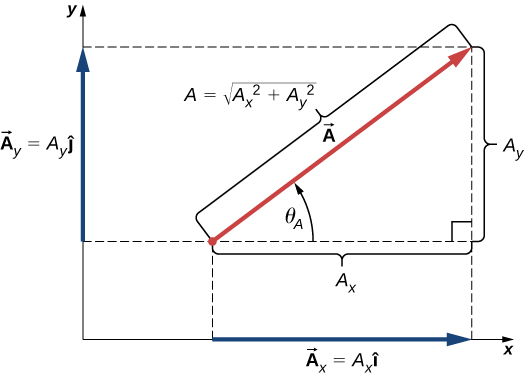
\includegraphics[width=0.33\textwidth]{vector1.jpeg} \hspace{0.5cm}
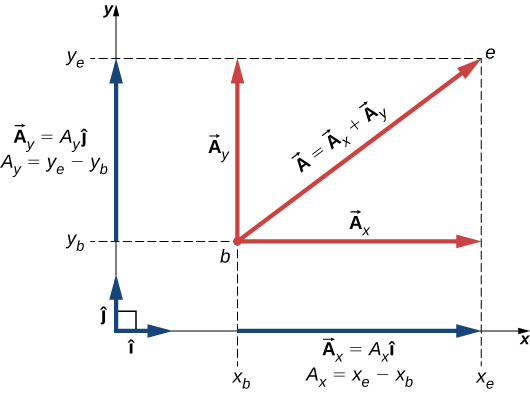
\includegraphics[width=0.33\textwidth]{vector2.jpeg}
\caption{\label{fig:1} A vector $\vec{A}$ can be expressed with components $A_x$ and $A_y$, or the magnitude $A = |\vec{A}|$ and the angle $\theta_A$.}
\end{figure}
\end{enumerate}

\end{document}
